\documentclass[10pt, a4paper]{article}
% ===== Essential Packages =====
\usepackage[utf8]{inputenc}       % UTF-8 encoding
\usepackage[T1]{fontenc}          % Better font encoding
\usepackage{lmodern}              % Modern Latin Modern font
\usepackage{ctex}                 % Chinese support (must be loaded after fontenc)
\usepackage{subcaption}
% ===== Math & Symbols =====
\usepackage{amsmath}              % Advanced math
\usepackage{amssymb}              % Additional math symbols
\usepackage{mathrsfs}             % Ralph Smith's Formal Script
\usepackage{braket}               % Dirac bra-ket notation
\usepackage{pdfpages}
% ===== Graphics & Tables =====
\usepackage{graphicx}             % Image support
\usepackage{float}                % Better float control
\usepackage{wrapfig}              % Wrapped figures
\usepackage{tikz}                 % Vector graphics
\usepackage[table]{xcolor}        % Colored tables
\usepackage{array}                % Enhanced tables
\usepackage{multirow}             % Multirow tables
\usepackage{tabularx}             % Adjustable-width tables
\usepackage{booktabs}             % Professional table lines
\usepackage{siunitx}              % SI units in tables
\usepackage{caption}              % Better captions
\usepackage{adjustbox}            % Box resizing
\usepackage{booktabs}
\usepackage{siunitx}
\usepackage{array}
\usepackage{makecell}
% ===== Code Listings =====
\usepackage{listings}             % Code blocks
\usepackage{tcolorbox}            % Colored boxes
\tcbuselibrary{listings, breakable} % Listings in tcolorbox

% ===== Misc =====
\usepackage{lipsum}               % Dummy text
\usepackage{footmisc}             % Better footnotes
\usepackage[margin=1in]{geometry} % Page margins
\usepackage{diagbox}
\usepackage{ctex}
\usepackage{multicol}  
\begin{document}
	\title{\vspace{-3.5cm}XRD}  % 向上移动标题
	\author{\vspace{-0.5cm}张世航}
	\date{} 
	\maketitle
	\section{吸收谱线}
	\begin{figure}[H]
		\centering
		
\includegraphics[width=0.7\linewidth]{XRD_with_peaks}
		\label{fig:xrdwithpeaks}
	\end{figure}
	\section{ZnO验证}
	\begin{figure}[H]
		\centering
		
\includegraphics[width=0.7\linewidth]{ZnO_XRD_Optimized_Layout}
		\label{fig:znoxrdoptimizedlayout}
	\end{figure}
	

\twocolumn  % 切换到双栏模式
	\begin{table}[htbp]
		\centering
		\caption{ZnO纤锌矿结构X射线衍射峰匹配分析结果}
		\label{tab:zno-xrd-peaks}
		\small
		\begin{tabular}{
				S[table-format=2.0]
				S[table-format=3.2]
				S[table-format=3.2]
				S[table-format=1.2]
				c
				S[table-format=4.0]
				S[table-format=1.3]
			}
			\toprule
			{\makecell{序号}} & 
			{\makecell{$2\theta_{\text{exp}}$\\ (\si{\degree})}} & 
			{\makecell{$2\theta_{\text{theo}}$\\ (\si{\degree})}} & 
			{\makecell{$\Delta 2\theta$\\ (\si{\degree})}} & 
			{(hkl)} & 
			{强度} & 
			{\makecell{误差\\ }} \\
			\midrule
			1  & 31.92 & 31.77 & 0.15 & 100 & 1981 & 0.472 \\
			2  & 34.56 & 34.42 & 0.14 & 002 & 1433 & 0.407 \\
			3  & 36.40 & 36.25 & 0.15 & 101 & 3241 & 0.414 \\
			4  & 47.68 & 47.54 & 0.14 & 102 &  661 & 0.294 \\
			5  & 56.72 & 56.60 & 0.12 & 110 & 1109 & 0.212 \\
			6  & 62.96 & 62.86 & 0.10 & 103 &  836 & 0.159 \\
			7  & 66.48 & 66.38 & 0.10 & 200 &  136 & 0.151 \\
			8  & 68.08 & 67.96 & 0.12 & 112 &  745 & 0.177 \\
			9  & 69.20 & 69.10 & 0.10 & 201 &  401 & 0.145 \\
			10 & 72.68 & 72.56 & 0.12 & 004 &   72 & 0.165 \\
			11 & 77.08 & 76.95 & 0.13 & 202 &  125 & 0.169 \\
			12 & 81.48 & 81.37 & 0.11 & 104 &   85 & 0.135 \\
			13 & 89.68 & 89.60 & 0.08 & 203 &  241 & 0.089 \\
			14 & 92.92 & 92.80 & 0.12 & 210 &   92 & 0.129 \\
			15 & 95.40 & 95.20 & 0.20 & 211 &  228 & 0.210 \\
			16 & 98.72 & 98.60 & 0.12 & 114 &  141 & 0.122 \\
			17 & 103.04 & 103.00 & 0.04 & 105 &  105 & 0.039 \\
			18 & 104.20 & 104.10 & 0.10 & 212 &  169 & 0.096 \\
			19 & 107.56 & 107.50 & 0.06 & 300 &   41 & 0.056 \\
			20 & 110.44 & 110.40 & 0.04 & 213 &  121 & 0.036 \\
			21 & 116.32 & 116.20 & 0.12 & 205 &  237 & 0.103 \\
			\bottomrule
		\end{tabular}
	\end{table}
	\section{理论分析}
    \begin{figure}[H]
    	\centering
    	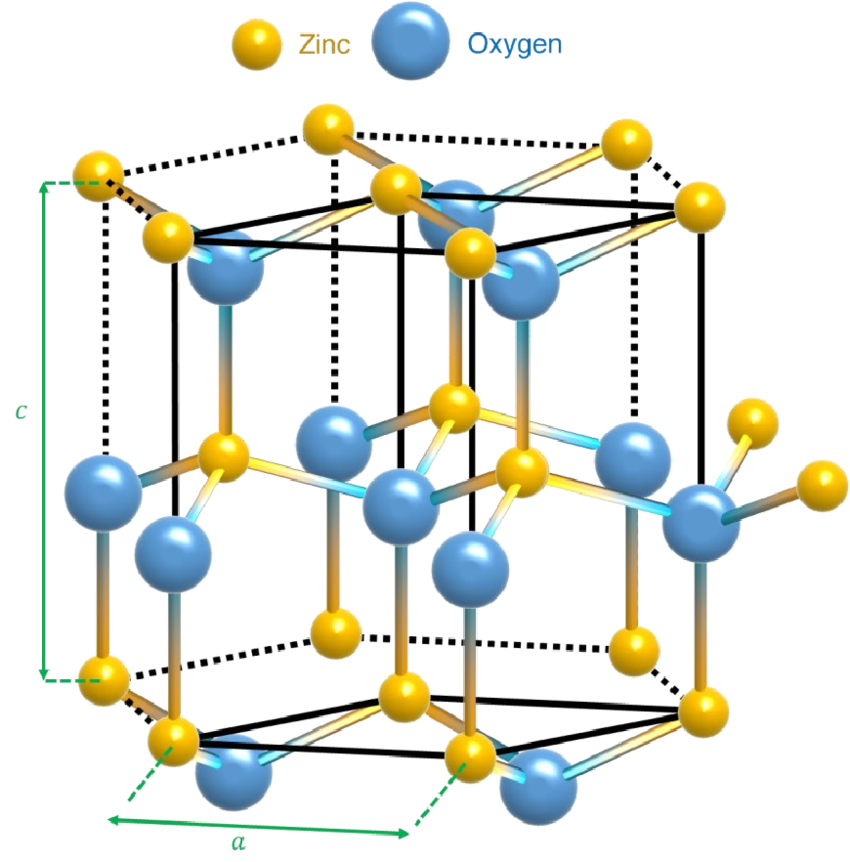
\includegraphics[width=0.7\linewidth]{llustration-of-the-structure-of-ZnO-The-yellow-and-blue-spheres-indicate-zin-and-oxygen}
    	\label{fig:llustration-of-the-structure-of-zno-the-yellow-and-blue-spheres-indicate-zin-and-oxygen}
    \end{figure}
    一个元胞内有6个$O$原子,6个$Zn$原子\\
    \[\textbf{K}_h = h_1\textbf{b}_1+h_2\textbf{b}_2+h_3\textbf{b}_3\]
    由于$\textbf{K}_h$垂直该族晶面,则它的法线方向可以写为$\textbf{e}_n = \frac{\textbf{K}_h}{|\textbf{K}_h|}$.\\
    则\[d_{h_1h_2h_3} = \textbf{e}_n\cdot\frac{1}{h_1}\textbf{a}_1=\frac{\textbf{K}_h\cdot\textbf{a}_1}{h_1|\textbf{K}_h|} = \frac{2\pi}{|\textbf{K}_h|}\]
	对于六角点阵初级矢量为
	\[\textbf{a} = (1,0,0)a\]
	\[\textbf{b} = (-\frac{1}{2},\frac{\sqrt{3}}{2},0)\]
	\[\textbf{c} = (0,0,1)c\]
	元胞体积为\[\Omega = \frac{\sqrt{3}}{2}a^2c\]
	倒空间基矢为\[\textbf{a}^*=\frac{4\pi}{\sqrt{3}a}(\frac{\sqrt{3}}{2}\textbf{i}+\frac{1}{2}\textbf{j})\]
    \[\textbf{b}^*=\frac{4\pi}{\sqrt{3}a}\textbf{j}\]
    \[\textbf{c}^*=\frac{2\pi}{c}\textbf{k}\]	
    倒空间的平移矢量为
    \[\textbf{K}_{hkl}=h\textbf{a}^*+k\textbf{b}^*+l\textbf{c}^*=\frac{2\pi}{a}h\textbf{i}+\frac{2\pi}{\sqrt{3}a}(h+2k)\textbf{j}+\frac{2\pi}{c}l\textbf{k}\]
	\[d_{hkl} =\frac{2\pi}{\sqrt{(2\pi)^2[(\frac{h}{a})^2+\frac{1}{3}(\frac{h+2k}{a})^2+(\frac{l}{c})^2]}}= \frac{1}{\sqrt{\frac{4}{3}(\frac{h^2+hk+k^2}{a^2}+\frac{l^2}{c^2})}}\]
    从劳厄方程出发
    \[\textbf{k}'-\textbf{k}=\textbf{K}_h\]
    两边平方,在$|\textbf{k}'=\textbf{k}|$的条件下,有\[-2\textbf{k}\cdot\textbf{K}_h=|\textbf{K}_h|^2\]
    \[\textbf{k}\cdot\frac{\textbf{K}_h}{|K_h|}=\frac{1}{2}|\textbf{K}_h|\]
    由此推导布拉格散射公式:\[\textbf{k}=\frac{2\pi}{\lambda}\]
    \[|\textbf{k}_h|=n\textbf{k}_h^*=n\frac{2\pi}{d}\]
    代入\[2\frac{1}{|\textbf{K}_h|}sin\theta=\frac{1}{|\textbf{k}|}\]
    可以得到\[2dsin\theta=n\lambda\]
    则 \[sin\theta = \frac{n\lambda}{2}\sqrt{\frac{4}{3}(\frac{h^2+hk+k^2}{a^2}+\frac{l^2}{c^2})}\]
    我们就得到了角度和晶面指数的关系.\\
    
\includepdf[pages=-, offset=0mm 0mm, scale=1.0]{Scan 06 1 26 16·55·18.pdf}
\end{document} 